\documentclass[12pt, a4paper]{article}
\usepackage[utf8]{inputenc}
\usepackage[T1]{fontenc}
\usepackage[slovene]{babel}
\usepackage{amsmath}
\usepackage{eurosym}
\usepackage{hyperref}
\usepackage{graphicx}
\usepackage[top=2.5cm, bottom=2.5cm, left=3cm, right=2.5cm]{geometry}
\usepackage{indentfirst}
\setlength{\parindent}{0.5cm}


\begin{document}

\begin{titlepage}
\begin{center}

\large
Univerza v Ljubljani\\
\normalsize
Fakulteta za matematiko in fiziko\\

\vspace{3 cm} 

\large
Žan Jernejčič in Ines Šilc\\

\vspace{0.5cm}
\LARGE
\textbf{Reševanje problema trgovskega potnika s k-optimalnim in
Lin-Kernighanovim algoritmom}

\vfill

\large Ljubljana, 2020

\end{center}
\end{titlepage}

\newpage

\section[Definiranje problema]{Definiranje problema}

V projektni nalogi bova reševala Problem trgovskega potnika s pomočjo k-optimalnega in Lin-Kernighanovega algoritma.\\

Problem trgovskega potnika oziroma Travelling salesman problem (krajše TSP) je problem, kjer imamo podanih $n$ mest in razdalje med vsemi (za vsak par mest imamo torej podano, koliko sta si oddaljeni). Zanima nas, ali lahko obiščemo vsako mesto in se na koncu vrnemo v prvotno mesto. Če označimo $d_{i, j}$ kot razdaljo mad $i$-tim in $j$-tim mestom, iščemo torej:

$$
\min_{\pi \in S_n} \sum\limits_{i=1}^{n-1} d_{\pi (i), \pi (i+1)} + d_{\pi (n), \pi (1)}
$$
 kjer je $S_n$ množica vseh permutacij danih $n$ mest. \\
 
Naivna rešitev je očitna, pogledamo $(n-1)!$ kombinacij, torej iz vsakega mesta v vsako drugo mesto, si zapišemo vse kombinacije in kakšno razdaljo smo prepotovali, ter izberemo tisto možnost, kjer je bila razdalja najkrajša.\\ 

Pred začetkom se lahko vprašamo kakšen mora biti graf, da lahko na njem izvajamo sledeča algoritma. Graf \textbf{ne sme} imeti \textbf{negativnih ciklov}, saj je najcenejši cikel potem očiten, in ustvarimo neskončno zanko, saj bo imela najboljša rešitev ceno -$\infty$. Ker imamo opravka s cikli, lahko cikel začnemo v kateremkoli vozlišču, zato lahko vedno gledamo možne poti od začetka.\\

Za projekt sva uporabila programski jezik \texttt{python}. Uporabljala sva naslednje pakete:

\begin{itemize}

\item \texttt{networkx}: za definiranje in generiranje grafov

\item \texttt{}

\item \texttt{}

\item \texttt{}

\item \texttt{}

\item \texttt{random}: za generiranje naključnih števil in seznamov

\item \texttt{matplotlib}: za izrisovanje grafov

\item \texttt{time}: za mertive časovne zahtevnosti

\item \texttt{itertools}: za generiranje prvotne permutacije

\end{itemize}

Za preverjanje veljavnosti poti v grafu za problem potujočega trgovca, morava vedeti:

\begin{itemize}

\item Vsaka pot trgovca bo morala imeti vsa vozlišča zato vedno preverimo:
\begin{center}
\texttt{pot.order() == originalen\_graf.order()}
\end{center}
\item Vsaka pot trgovca bo morala imeti točno toliko povezav kot vozlišč:
\begin{center}
\texttt{pot.size(weight = None) == pot.order()} 
\end{center}
\item Dolžina poti: \texttt{pot.size()}

\end{itemize}











\newpage
\section[k-optimalni algoritmi]{k-optimalni algoritmi}

K-optimalni algoritem, je lokalni algoritem, kjer iščemo rešitev Problema trgovskega potnika in sorodnih problemov. Algoritem deluje tako, da zmanjša dolžino trenutnega potovanja, dokler ne dosežemo poti, katere dolžine ne moremo izboljšati.\\

Poznamo dve glavni različici k-opt algoritma, to sta 2-Opt in 3-Opt algoritem. 2-Opt algoritem deluje tako, da odstrani dve vozlišči grafa (dve mesti), tako razdeli pot na dva dela, poišče najboljšo rešitev podproblema, in nato poveže nazaj mesti na najboljši možen način. 3-Opt algoritem odstrani tri povezave ali vozlišča, tako dobimo 3 podomrežja mest. V naslednjem koraku analiziramo najboljšo pot med temi tremi podomrežji. To ponavljamo za druge tri povezave, dokler nismo poskusili vseh možnih poti v danem omrežju.

\subsection[2-opt algoritem]{2-opt algoritem}

\begin{verbatim}

def dva_opt(graf, pot):

    najboljsa_pot = pot

    izboljsanje = True
    while izboljsanje:
        izboljsanje = False
        for i in range(1, len(pot) - 2):

            for j in range(i + 1, len(pot)):

                if j - i == 1: continue
                nova_pot = pot
                nova_pot[i:j] = pot[j - 1:i - 1:-1]

                if cena_poti(graf, nova_pot) < cena_poti(graf, najboljsa_pot):
                    najboljsa_pot = nova_pot
                    izboljsanje = True
        pot = najboljsa_pot

    return (pot, cena_poti(graf, pot))

\end{verbatim}

\begin{figure}[!h]
    
    \begin{minipage}{0.5\textwidth}
    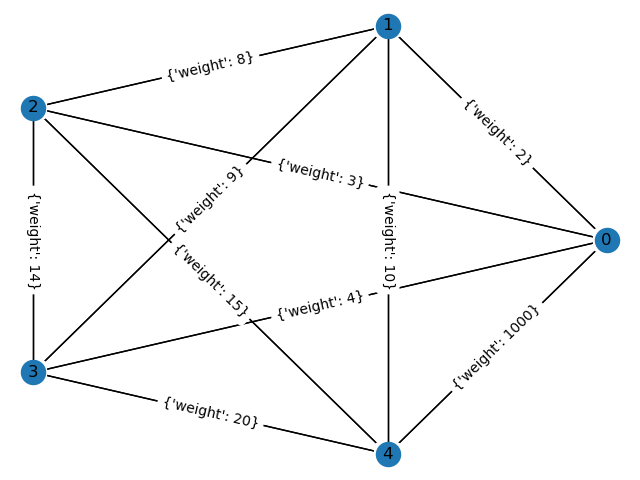
\includegraphics[width=8 cm]{primer.png}
    \caption{Primer}
    \label{primer_2_opt}
  \end{minipage}
 \hspace{1cm}
  \begin{minipage}{0.5\textwidth}
    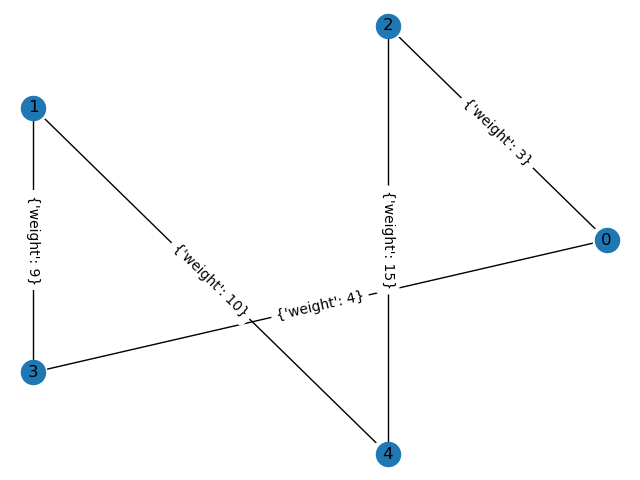
\includegraphics[width=8 cm]{resitev_primer.png}
    \caption{Rešitev}
    \label{resitev_2_opt}
  \end{minipage}
    
\end{figure}

\subsection[3-opt algoritem]{3-opt algoritem}

\newpage
\section[Lin-Kernighanov algoritem]{Lin-Kernighanov algoritem}

\newpage
\section[Viri]{Viri}

\begin{enumerate}

\item A. Hagberg, D. Schult, P. Swart:\emph{NetworkX Refrence, Release 2.4}, [ogled 2.~1.~2020], dostopno na \url{https://networkx.github.io/documentation/stable/_downloads/networkx_reference.pdf}

\end{enumerate}

\end{document}